\documentclass[10pt,a4paper]{article}
\usepackage[margin=1.9cm]{geometry}
\usepackage[T1]{fontenc}
\usepackage{lmodern}
\usepackage{microtype}
\usepackage{graphicx}
\usepackage{booktabs}
\usepackage{array}
\usepackage{float}
\usepackage{caption}
\usepackage{enumitem}
\usepackage{tikz}
\usetikzlibrary{arrows.meta,positioning,fit,backgrounds,shapes.geometric,calc}
\usepackage[hidelinks]{hyperref}
\setlist{itemsep=2pt,topsep=4pt}
\setlength{\parskip}{3pt}
\setlength{\parindent}{0pt}
\setlength{\emergencystretch}{2em}
\captionsetup{font=small,labelfont=bf,skip=3pt}
\setlength{\textfloatsep}{8pt}\setlength{\floatsep}{6pt}\setlength{\intextsep}{6pt}
\graphicspath{{figures/}}
\newcommand{\code}[1]{\texttt{#1}}
\newcommand{\fig}[3][0.9]{\begin{figure}[H]\centering\includegraphics[width=#1\linewidth]{#2}\caption{#3}\end{figure}}
\newcommand{\twofig}[3]{\begin{figure}[H]\centering\includegraphics[width=0.49\linewidth]{#1}\hfill\includegraphics[width=0.49\linewidth]{#2}\caption{#3}\end{figure}}
\newcolumntype{R}[1]{>{\raggedright\arraybackslash}p{#1}}

\newcommand{\teammembers}{Team 97\\[6pt]\normalsize\begin{tabular}{ll}
Ahmed Tamer Mohamed Hany Saleh Elmeazawy & 58-14045\\
Youssef Mohamed Mohamed Elkhodary & 58-18247\\
Omar Gamaleldin Mohamed Abdelbaky & 58-13583\\
Omar Hisham Abdelrahman Mahrous Abdelrahman & 58-25441
\end{tabular}}

\title{Formula 1 Graph-RAG Assistant\\\large Milestone 3 report}
\author{\teammembers}
\date{November 2026}

\begin{document}
\maketitle

\noindent Every number in this report is read from a file written by the evaluation scripts in \code{milestone3/eval/} (results in \code{milestone3/eval/results/}) or from \code{milestone3/models/meta.json}. Where we computed a small extra figure from those files we say so.

%==============================================================
\section{Introduction}

The assistant answers Formula~1 questions in a chat window and explains podium predictions. It joins two kinds of knowledge. The \emph{symbolic} part is the Neo4j knowledge graph of Milestone~2 (14 source tables, 1950--2024): every factual answer comes from a fixed, parameterised Cypher template, and the language model only puts the returned rows into one to three sentences. It never writes Cypher and never sees the graph. The \emph{statistical} part is the shallow neural network of Milestone~1, which gives a podium probability from nine pre-race features, a live SHAP explanation of that probability, and a language model that turns the SHAP numbers and a few pre-race graph facts into plain language. Questions and predictions share one graph and one interface, and the graph schema is unchanged from Milestone~2.

%==============================================================
\section{System architecture}

Figure~\ref{fig:arch} shows both paths. A chat message is classified (rules first, sentence-embedding fallback), its entities are extracted and merged with the session cache, one template is run on the graph, and two language models answer the same prompt side by side. A prediction question is handed over to the prediction view, which prefills the nine features from the Milestone~1 model table, runs the saved network, computes SHAP live, queries the graph for facts strictly before the race date and asks one language model to explain the result.

\begin{figure}[t!]
\centering
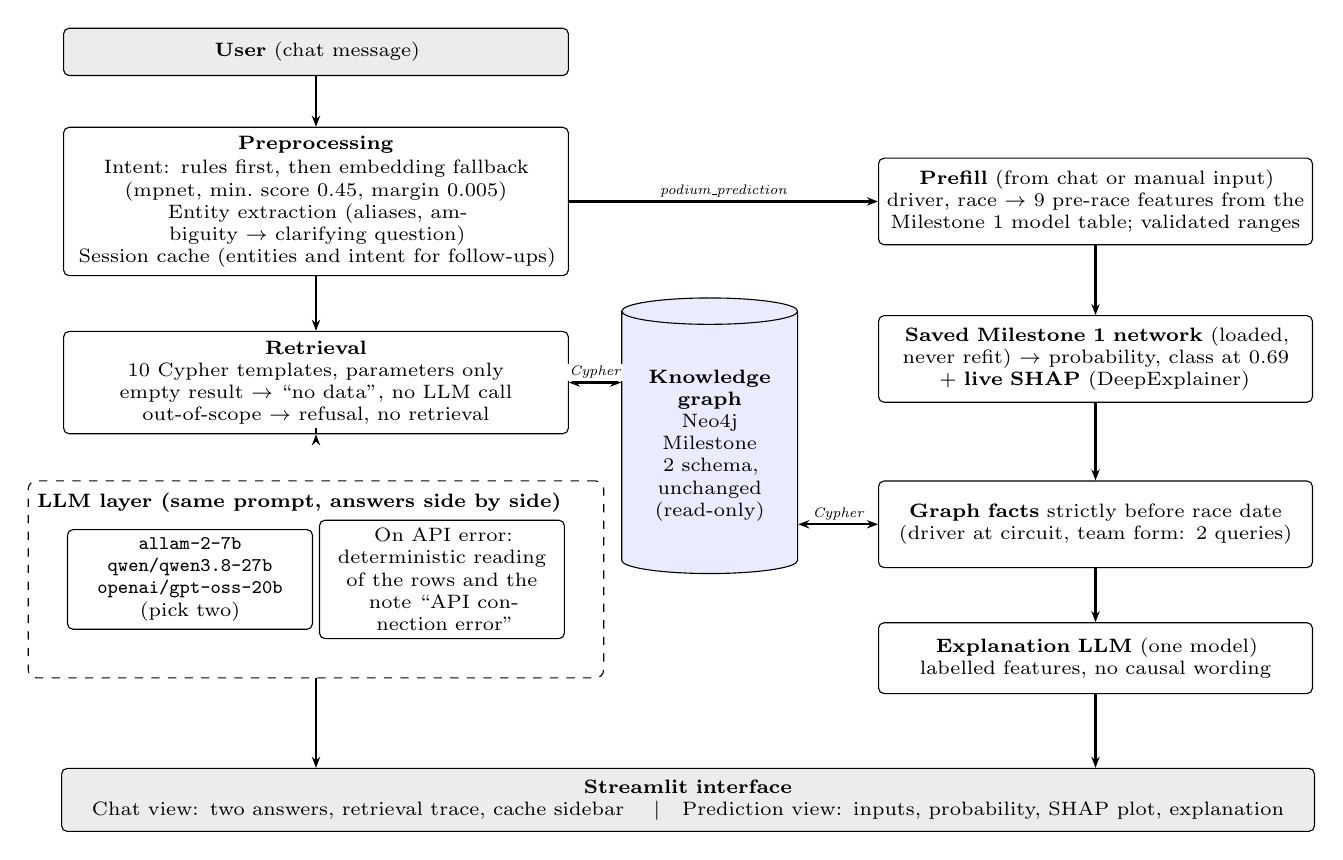
\begin{tikzpicture}[
  font=\scriptsize,
  box/.style={draw,rounded corners=2pt,align=center,fill=white,inner sep=3pt},
  lbox/.style={box,text width=6.2cm},
  rbox/.style={box,text width=5.3cm},
  arr/.style={-{Stealth[length=4pt]},thick},
  darr/.style={{Stealth[length=4pt]}-{Stealth[length=4pt]},thick},
  lab/.style={font=\tiny\itshape,fill=white,inner sep=1pt}]
% chat path (left)
\node[box,fill=gray!15,minimum height=0.6cm,text width=6.2cm] (user) at (0,0) {\textbf{User} (chat message)};
\node[lbox,minimum height=1.7cm] (pre) at (0,-1.9) {\textbf{Preprocessing}\\[1pt]
 Intent: rules first, then embedding fallback\\(mpnet, min.\ score 0.45, margin 0.005)\\
 Entity extraction (aliases, ambiguity $\rightarrow$ clarifying question)\\Session cache (entities and intent for follow-ups)};
\node[lbox,minimum height=1.3cm] (ret) at (0,-4.2) {\textbf{Retrieval}\\10 Cypher templates, parameters only\\empty result $\rightarrow$ ``no data'', no LLM call\\out-of-scope $\rightarrow$ refusal, no retrieval};
\node[box,text width=2.9cm,minimum height=0.9cm] (llmA) at (-1.6,-6.7) {\code{allam-2-7b}\\\code{qwen/qwen3.8-27b}\\\code{openai/gpt-oss-20b}\\(pick two)};
\node[box,text width=2.9cm,minimum height=0.9cm] (llmB) at (1.6,-6.7) {On API error:\\deterministic reading\\of the rows and the\\note ``API connection error''};
\begin{scope}[on background layer]
\node[draw,dashed,rounded corners=3pt,fit=(llmA)(llmB),inner sep=14pt,label={[font=\scriptsize\bfseries,anchor=north west,yshift=-1pt]north west:LLM layer (same prompt, answers side by side)}] (llm) {};
\end{scope}
% knowledge graph (centre)
\node[draw,cylinder,shape border rotate=90,aspect=0.15,minimum height=3.5cm,text width=2.0cm,align=center,fill=blue!8] (kg) at (5.0,-5.0) {\textbf{Knowledge graph}\\Neo4j\\Milestone 2 schema,\\unchanged\\(read-only)};
% prediction path (right)
\node[rbox,minimum height=1.1cm] (pf) at (9.9,-1.9) {\textbf{Prefill} (from chat or manual input)\\driver, race $\rightarrow$ 9 pre-race features from the\\Milestone 1 model table; validated ranges};
\node[rbox,minimum height=1.1cm] (nn) at (9.9,-3.9) {\textbf{Saved Milestone 1 network} (loaded,\\never refit) $\rightarrow$ probability, class at 0.69\\+ \textbf{live SHAP} (DeepExplainer)};
\node[rbox,minimum height=1.1cm] (gf) at (9.9,-6.0) {\textbf{Graph facts} strictly before race date\\(driver at circuit, team form: 2 queries)};
\node[rbox,minimum height=0.9cm] (ex) at (9.9,-7.7) {\textbf{Explanation LLM} (one model)\\labelled features, no causal wording};
% interface
\node[box,fill=gray!15,minimum height=0.8cm,text width=15.7cm] (ui) at (4.725,-9.5) {\textbf{Streamlit interface}\\Chat view: two answers, retrieval trace, cache sidebar \quad$|$\quad Prediction view: inputs, probability, SHAP plot, explanation};
% arrows
\draw[arr] (user) -- (pre);
\draw[arr] (pre) -- (ret);
\draw[arr] (ret) -- (llm.north |- ret.south);
\draw[arr] (pre.east) -- node[lab,above] {podium\_prediction} (pf.west);
\draw[arr] (pf) -- (nn);
\draw[arr] (nn) -- (gf);
\draw[arr] (gf) -- (ex);
\draw[darr] (ret.east) -- node[lab,above] {Cypher} (ret.east -| kg.west);
\draw[darr] (gf.west) -- node[lab,above] {Cypher} (gf.west -| kg.east);
\draw[arr] (llm.south) -- (llm.south |- ui.north);
\draw[arr] (ex.south) -- (ex.south |- ui.north);
\end{tikzpicture}
\caption{Architecture. Left: the chat path. Right: the separate prediction path. Both read the same knowledge graph; the graph is queried only through fixed templates and two fixed fact queries.}\label{fig:arch}
\end{figure}

Everything a turn does is logged as one JSON line, and every prediction explanation is logged as well (message, intent and which stage decided it, entities, template, Cypher, parameters, rows, prompt, answer, model, latency, tokens). Failures of the graph (Neo4j down) or of a language-model call never raise into the interface: the user sees ``Neo4j is not reachable'' or ``API connection error'' plus the deterministic reading of the rows.

%==============================================================
\section{Question types and examples}\label{sec:types}

Table~\ref{tab:intents} lists the twelve intents: ten retrieval intents (one or more templates each), the prediction intent and the out-of-scope intent. ``Hops'' is the number of relationships on the longest path of the template's \code{MATCH} pattern (the paths are listed below the table). ``Graphical'' templates return Neo4j paths, from which the interface draws the subgraph (nodes, edges, relationship statements); ``scalar'' templates return aggregates, and the interface shows the value only. The results in the table are the first row the template returns for the example, read from the running graph.

\begin{table}[t!]
\centering\scriptsize\setlength{\tabcolsep}{3pt}
\caption{The twelve intents, the entities each needs (optional ones in brackets), one example and the result of the matching template.}\label{tab:intents}
\begin{tabular}{@{}R{1.9cm}R{1.5cm}R{1.6cm}R{3.6cm}R{4.6cm}cR{1.0cm}@{}}
\toprule
Intent & Family & Entities & Example phrasing & Result of the template & Hops & Output \\
\midrule
driver\_\allowbreak{}season\_\allowbreak{}stats & Driver performance & driver [year(s)] & How many wins did Lewis Hamilton have in 2019? & 21 races, 11 wins, 17 podiums, 413 points, 21 classified & 2 & scalar \\
driver\_\allowbreak{}circuit\_\allowbreak{}record & Driver performance & driver, circuit [years] & How many times has Lewis Hamilton won at Silverstone before 2020? & 13 starts (2007--2019), 6 wins, 9 podiums, best finish 1, mean finish 3.46 & 3 & scalar \\
constructor\_\allowbreak{}stats & Constructor performance & constructor [years] & How reliable was Ferrari between 2014 and 2021? & 320 entries, 277 classified (reliability 0.866), 17 wins, 100 podiums & 2 & scalar \\
head\_\allowbreak{}to\_\allowbreak{}head & Head-to-head & driver, driver2 [constructor, years] & Lewis Hamilton vs Bottas: who finished ahead more often? & 246 shared races: Hamilton ahead 205, Bottas ahead 41; plus the 10 latest shared races & 4 & graphical \\
race\_\allowbreak{}result & Race and circuit facts & race or circuit, year & Who won the 2019 British Grand Prix? & P1 Lewis Hamilton (Mercedes, grid 2, 26 points); top 10 finishers & 3 & graphical \\
circuit\_\allowbreak{}info & Race and circuit facts & circuit & Where is Silverstone and how many races were held there? & Silverstone, UK, altitude 153 m, 59 races, 1950--2024, two Grand Prix names & 1 & scalar \\
qualifying\_\allowbreak{}record & Qualifying and grid & driver [year(s)] & How many poles did Max Verstappen get in 2022? & 22 sessions, 8 poles, 15 front rows, mean qualifying position 2.59 & 2 & scalar \\
grid\_\allowbreak{}gains & Qualifying and grid & race or circuit, year & Who gained the most places at the 2021 Italian Grand Prix? & Valtteri Bottas, grid 19 to P3, +16 places; top 5 & 3 & graphical \\
pit\_\allowbreak{}stops & Pit stops and strategy & race or circuit, year [driver] & Who had the fastest pit stop at the 2023 Monaco Grand Prix? & Pierre Gasly, 23.902 s on lap 47; five fastest stops (driver variant lists a driver's stops) & 3 (2) & graphical \\
season\_\allowbreak{}standings & Season and history & year & Who won the 2021 championship? & Max Verstappen, 388.5 race points, 10 wins; top 10, 21 drivers & 3 & scalar \\
podium\_\allowbreak{}prediction & Prediction view & driver [race, year, feature values] & Predict Lando Norris at the 2024 Miami Grand Prix & no template: opens the prediction view with the fields prefilled & --- & --- \\
out\_\allowbreak{}of\_\allowbreak{}scope & Refusal & --- & What is the capital of France? & fixed refusal; no retrieval, no trace, cache untouched & --- & --- \\
\bottomrule
\end{tabular}
\end{table}

{\sloppy \textbf{Hops.} The longest paths are: \code{Driver<-\allowbreak{}Result->\allowbreak{}Race->\allowbreak{}Circuit} (driver\_circuit\_record, grid\_gains), \code{Driver<-\allowbreak{}Result->\allowbreak{}Race<-\allowbreak{}Result->\allowbreak{}Driver} (head\_to\_head, 4), \code{Circuit<-\allowbreak{}Race<-\allowbreak{}Result->\allowbreak{}Driver} (race\_result), \code{Driver<-\allowbreak{}PitStop->\allowbreak{}Race->\allowbreak{}Circuit} (pit\_stops), \code{Driver<-\allowbreak{}Result->\allowbreak{}Race->\allowbreak{}Season} (season\_standings), \code{Driver<-\allowbreak{}Result->\allowbreak{}Race} (driver\_season\_stats, qualifying\_record via \code{Qualifying}, constructor\_stats via \code{Constructor}) and \code{Circuit<-\allowbreak{}Race} (circuit\_info). Nine of the ten retrieval intents cross two or more hops and six cross three or more (driver\_circuit\_record, head\_to\_head, race\_result, grid\_gains, pit\_stops, season\_standings), against the required three.}

\textbf{New relative to Milestone 2.} Six intents are entirely new: driver\_season\_stats, race\_result, circuit\_info, qualifying\_record, grid\_gains and pit\_stops. Four more generalise the first four Milestone~2 queries into parameterised templates (season\_standings from Query~1, constructor\_stats from Query~2, head\_to\_head from Query~3, driver\_circuit\_record from Query~4); Query~5 (drivers who changed team) has no template. Intents that take more than one entity: head\_to\_head (two drivers and an optional team), driver\_circuit\_record (driver, circuit, optional years), race\_result, grid\_gains and pit\_stops (race or circuit plus year, pit\_stops with an optional driver); the requirement is two.

\textbf{Template design.} Every value is a Cypher parameter; optional slots are handled inside the query (\code{\$year\_from IS NULL OR ...}), so one template serves ``at Silverstone'', ``before 2020'' and ``since 2015''. Entries that never started (\emph{Did not qualify}, \emph{Did not prequalify}, \emph{Withdrew}) are excluded. Every template ends with a \code{LIMIT} or an aggregation and returns named columns, plus a one-sentence scope (what the data covers and excludes) that the model is told to repeat.

\textbf{Empty results and refusals.} If a template returns no rows the pipeline answers with a fixed ``no data'' message and does not call a model, so the model is never asked to fill the gap from memory. The test set has seven such items, for example the 2025 championship (the data ends in 2024), the fastest pit stop at the 2005 Monaco Grand Prix (pit stops start in 2011) and Senna's poles in 1985 (qualifying starts in 1994); all seven were handled correctly (Table~\ref{tab:pipeline}). Out-of-scope questions (weather, tyres, other topics, such as the capital of France) are refused before any retrieval and the session cache is left untouched.

%==============================================================
\section{Intent classification}

\textbf{Approaches.} (1) \emph{Rules}: an ordered list of regular expressions per intent, first match wins, out-of-scope patterns first (so that ``weather at Silverstone'' is refused before the track name routes it to a circuit intent). (2) \emph{Embeddings}: each intent has 10--12 example phrasings, embedded once with a sentence-transformer; a question is assigned to the intent of its most similar example (maximum per intent, because the examples of one intent are deliberately diverse). The classifier says ``rephrase'' instead of guessing when the best cosine similarity is below a minimum score or the margin to the second-best intent is below a minimum margin. An out-of-scope decision is never made by similarity alone: if the embedding winner is out\_of\_scope but the text contains Formula~1 vocabulary and the rules do not agree, the result is ``rephrase'', as the specification requires. Two hybrids combine them (rules first or embeddings first).

\textbf{Labelled set.} 94 questions, 7--10 per intent (including out-of-scope), worded differently from the classifier examples. ``Rephrase'' counts as wrong and is its own column in the confusion matrices.

\textbf{Embedding model and thresholds.} Three Hugging Face models were benchmarked; for each, the two thresholds were chosen by \emph{leave-one-out} on the classifier's own examples (each example is classified against all the others over a grid of score and margin values; we take the most precise pair whose rephrase rate stays at or below 10\%). Nothing is tuned on the labelled set. The model winner is the one with the best leave-one-out precision, which is also the one with the best accuracy on the labelled set (Table~\ref{tab:embed}).

\begin{table}[H]
\centering\small
\caption{Embedding models. Precision is leave-one-out on the classifier examples; accuracy and rephrase rate are on the 94 labelled questions.}\label{tab:embed}
\begin{tabular}{lcccccc}
\toprule
Model & min.\ score & min.\ margin & LOO precision & accuracy & rephrase rate \\
\midrule
\code{all-MiniLM-L6-v2} & 0.300 & 0.005 & 0.355 & 0.532 & 0.085 \\
\code{all-mpnet-base-v2} (winner) & 0.450 & 0.005 & 0.518 & 0.787 & 0.085 \\
\code{bge-small-en-v1.5} & 0.300 & 0.000 & 0.270 & 0.532 & 0.011 \\
\bottomrule
\end{tabular}
\end{table}

\textbf{Results.} Table~\ref{tab:intent} gives the accuracy of the four classifiers; Figures~\ref{fig:cm1} and~\ref{fig:cm2} give the confusion matrices of the rule-based, the embedding and the deployed hybrid classifier. The last two columns split the 94 questions into the first 70 and the last 24 rows of the file (computed from \code{intent\_predictions.csv}), see the caveat below.

\begin{table}[H]
\centering\small
\caption{Intent classification on the 94 labelled questions.}\label{tab:intent}
\begin{tabular}{lcccc}
\toprule
Approach & accuracy (correct/94) & rephrase rate & first 70 & last 24 \\
\midrule
Rules & 0.915 (86) & 0.043 & 67/70 & 19/24 \\
Embeddings (mpnet) & 0.787 (74) & 0.085 & 55/70 & 19/24 \\
Hybrid, rules first (\textbf{deployed}) & \textbf{0.936} (88) & 0.011 & 68/70 & 20/24 \\
Hybrid, embeddings first & 0.862 (81) & 0.011 & 59/70 & 22/24 \\
\bottomrule
\end{tabular}
\end{table}

\twofig{intent_confusion_rule}{intent_confusion_embedding}{Confusion matrices (rows true, columns predicted; last column ``rephrase''): rule-based (left) and embedding classifier (right).\label{fig:cm1}}

\fig[0.5]{intent_confusion_hybrid}{Confusion matrix of the deployed hybrid: rules first, embeddings as fallback.\label{fig:cm2}}

\textbf{What is deployed, and why.} The rule-first hybrid: it has the best accuracy on the labelled set (0.936) and the lowest error, rules answer the common wordings exactly and instantly and can be read and debugged, and the embedding classifier handles only what the rules miss (it generalises to new wordings but confuses neighbouring intents such as constructor and driver statistics). In the application the order is: rules, then the follow-up rule (a message starting with ``and'', ``what about'', ``how about'', ``also'', ``then'' or ``same for'', or of at most six words that names an entity, keeps the cached intent), then the embedding classifier, then ``please rephrase''. The six errors of the hybrid are: ``Brawn in 2009'' (constructor routed to race\_result), ``average finishing position at Estoril'' and ``how many races did Toyota win'' (routed to driver\_season\_stats), a Villeneuve-or-Frentzen question (head\_to\_head routed to constructor\_stats), and two out-of-scope questions (``How do I cook pasta?'' became ``rephrase'', ``How many people watch Formula 1 on TV?'' became circuit\_info).

\textbf{Honesty about the rule set.} The rules were partly tuned on the first 70 questions, so their 67/70 on that part is optimistic. The last 24 questions were written afterwards, as fresh questions, to check this: the rules score only 19/24 (0.792) there and the hybrid 20/24 (0.833). After scoring them we changed the rules further, so neither part is a clean held-out set any more, and the overall 0.915 and 0.936 should be read as upper estimates. The embedding classifier is not affected by this (its thresholds came from the classifier examples only), and it scores 19/24 on the fresh part as well.

%==============================================================
\section{Entity extraction and session}

\textbf{Extraction.} Look-up tables (drivers with first and last season, constructors, circuits, race names) are read from the graph once at start-up. Matching is case- and accent-insensitive on whole words, over phrases of up to six words; when matches overlap the longest wins (ties: race, circuit, constructor, driver), so ``Red Bull Ring'' is a circuit rather than the team and ``Miami Grand Prix'' is a race rather than the circuit Miami. Drivers match by full name, by surname (three letters or more, not a common word) and by upper-case three-letter code if unique; teams by name, short form and hand-written aliases (``merc'', ``rb''); circuits by name, city and aliases (``COTA''); a country names a circuit only if it has exactly one. Years are read as a single season, a range (``2014 to 2021''), or an open range (``before 2020'' $\rightarrow$ up to 2019, ``since 2015'').

\textbf{Ambiguity.} A name with several records is never guessed. ``Hamilton'' maps to Lewis and Duncan Hamilton, ``Schumacher'' to Michael, Ralf and Mick, and the assistant asks ``Which Hamilton do you mean: Lewis or Duncan?''. This is a team decision: a shared surname always triggers the question unless a year in the message narrows the candidates to the drivers who were active then (``Schumacher in 2022'' resolves to Mick). The open question is stored in the session; the next message answers it if it names a candidate, otherwise it is processed as a fresh question. A missing required slot is asked for in the same way (``Which driver do you mean?'').

\textbf{Cache rules.} The session keeps the last intent and the last entities. A new message replaces only the slots it names; the season slots (\code{year}, \code{year\_from}, \code{year\_to}) are one group, so naming any of them replaces all three. The follow-ups of the specification work as follows (the cache is shown in the sidebar):
\begin{itemize}
\item ``And in 2020?'' keeps the driver or team and replaces the season.
\item ``What about Norris?'' keeps the season and replaces the driver.
\item ``2021?'' and ``How many points did he score in 2019?'' reuse the cached driver (there is no pronoun resolver: the driver slot is simply absent from the message, so the cached one is used).
\item ``And at Monza?'' after Hamilton at Silverstone before 2020 keeps driver and years and replaces the circuit.
\end{itemize}
After an explicit change of intent only the \emph{required} slots of the new intent are carried over, so a driver from an earlier question is not silently applied to ``fastest pit stops at Monaco in 2019''. In a head-to-head conversation, a follow-up that names one driver (``And against Rosberg?'') replaces the \emph{opponent} and keeps the first driver. An out-of-scope question returns before the cache is merged, so neither the cache nor the cached intent is cleared and ``And in 2018?'' still works afterwards.

%==============================================================
\section{Podium prediction explainer}

\textbf{The model.} The network is the Milestone~1 shallow neural network (two hidden layers of 64 and 32 units, dropout 0.2, weight decay $10^{-4}$, positive-class weight 6.44). The Milestone~1 notebook never saved its model, so we added a final cell (section~18) that re-runs the network in the same notebook and exports the fitted preprocessor (median imputation and scaling fitted on the training seasons), the weights, the 200-row SHAP background used in Milestone~1, the Milestone~1 global SHAP importances and \code{meta.json}. The cell also saves a copy of the pre-race feature table as \code{models/model\_table.csv}, so that a fresh clone does not need the Milestone~1 \code{outputs/} folder. The application loads these files; nothing is fitted or refitted in the application. The threshold, 0.69, is the one that maximised F1 on the validation seasons (2020--2021) in the exported run.

\textbf{Why 0.69 and not the 0.78 of the Milestone~1 report.} The export re-ran the training, and the re-run selected the learning rate 0.001 instead of 0.003 (network results depend slightly on the seed and the PyTorch version). A different network has a different validation-optimal threshold, so the saved threshold is 0.69. Ranking quality is the same: test PR-AUC 0.713 (\code{meta.json}: 0.7129) against 0.714 in the Milestone~1 README; test ROC-AUC 0.941 in both. The saved run has validation PR-AUC 0.742 and test F1 0.683 (precision 0.566, recall 0.863). The application uses the saved model with its own saved threshold. Probabilities are not calibrated and should be read as ranking scores.

\textbf{Pre-race features and leakage.} The nine features come from the Milestone~1 model table, built with the Milestone~1 leakage rules (cutoff after qualifying; the grid, the qualifying result, the standings after the previous round and the form from earlier races are known before the start; nothing from the race itself). The standings are not in the graph, and we did not add them: the graph schema is unchanged and the standings come from the Milestone~1 table.

\textbf{Manual input design.} The prediction view can be reached from the chat (driver, race and year prefilled) or entered by hand. Each feature has one input, with its meaning and valid range in the help text. Valid ranges are the observed minimum and maximum in the Milestone~1 model table (24,724 driver-races, 1950--2024), with shares limited to 0--1: a value outside has never happened, so the network would be extrapolating. Defaults are the training-season medians, which is what the Milestone~1 imputer fills. A value that is missing, not a number, not whole where it must be, or outside the range produces an error naming the field and no probability is computed (the predictor checks again and raises).

\begin{table}[H]
\centering\scriptsize
\caption{The nine inputs. Range = observed minimum to maximum (\code{feature\_ranges.csv}); the 1\%--99\% range is given as evidence that the extremes are rare.}\label{tab:features}
\begin{tabular}{@{}R{2.9cm}R{1.5cm}R{1.5cm}cR{1.7cm}R{6.0cm}@{}}
\toprule
Feature (code) & Input & Valid range & Default & 1\%--99\% & Help text (meaning) \\
\midrule
Starting grid position (\code{grid\_pos}) & whole number & 1--34 & 12 & 1--26 & Where the driver lines up (1 = pole); a pit-lane start counts as the back of the field. \\
Pit-lane start (\code{pit\_lane\_start}) & checkbox 0/1 & 0--1 & 0 & 0--0 & 1 if the driver starts from the pit lane. \\
Qualifying position (\code{quali\_pos}) & whole number & 1--26 & 11 & 1--24 & Position in qualifying (1 = fastest); can differ from the grid after penalties. \\
Q1 gap to the fastest (\code{q1\_gap\_pct}) & decimal, \% & 0--44.8 & 1.5 & 0--8.65 & How much slower the Q1 lap was than the fastest Q1 lap (0 = fastest). \\
Driver championship position (\code{drv\_standing}) & whole number & 1--102 & 12 & 1--42 & Place in the championship after the previous round (1 = leader). \\
Team championship position (\code{con\_standing}) & whole number & 1--20 & 6 & 1--16 & Team's place in the constructors' championship after the previous round. \\
Recent podium rate (\code{drv\_podium\_last}) & decimal, share & 0--1 & 0 & 0--1 & Share of the last 3 races on the podium (0, 0.33, 0.67 or 1). \\
Recent finishing level (\code{drv\_finish\_last}) & decimal, share & 0--1 & 0.53 & 0.06--0.92 & Mean finishing place of the last 3 races as a share of the field (near 0 = front). \\
Career podium rate (\code{drv\_career\_podium}) & decimal, share & 0--1 & 0.05 & 0--0.62 & Share of all earlier races on the podium. \\
\bottomrule
\end{tabular}
\end{table}

\textbf{Live SHAP.} For one row, \code{shap.DeepExplainer} is run on the saved network with the saved 200-row Milestone~1 background. Contributions are in log-odds (the network output before the sigmoid): the base value ($-1.763$) plus the nine contributions equals the log-odds of the prediction. Their sizes rank the features; they are not percentage points and not causes. The interface shows the waterfall plot (Figure~\ref{fig:waterfall}) next to the language-model explanation.

\textbf{Graph facts, strictly before the race.} Two Cypher queries add context to the explanation: the driver's earlier starts, wins, podiums and best finish at this circuit, and the team's not-finished and podium counts in the three preceding years. Both filter on \code{race.date < date(\$raceDate)}, so the race itself is never counted. If Neo4j fails, the explanation is produced without facts.

\textbf{Explanation cases.} Table~\ref{tab:cases} lists the nine driver-and-race cases (the requirement is five, with one predicted podium and one non-predicted). Five are predicted podiums and four are not. The prediction matches the actual outcome in six of nine; the three misses are shown in the table and are ranking-model errors, not interface errors: Hamilton in Austria 2022 (0.64, just under the threshold) and Gasly in the Netherlands 2023 finished on the podium although the model said no, and Verstappen in Bahrain 2022 was predicted on the podium (0.94, driven by the grid position) but finished 19th. The numbers come from the predictor self-test (\code{python -m milestone3.prediction.predictor}).

\begin{table}[H]
\centering\small
\caption{Explanation cases: predicted probability (threshold 0.69), predicted class, actual finish and the three largest SHAP contributions (log-odds).}\label{tab:cases}
\begin{tabular}{@{}R{2.9cm}R{2.3cm}clllR{5.6cm}@{}}
\toprule
Driver & Race & $p$ & Class & Actual & Match & Largest contributions \\
\midrule
Max Verstappen & Monaco 2023 & 0.96 & podium & P1 & yes & grid +2.24, recent podiums +1.08, career podiums +0.71 \\
Lando Norris & Hungary 2024 & 0.93 & podium & P2 & yes & grid +2.23, recent podiums +0.68, qualifying +0.58 \\
Charles Leclerc & Miami 2024 & 0.91 & podium & P3 & yes & grid +2.36, team standing +0.56, career podiums +0.41 \\
Max Verstappen & Miami 2023 & 0.74 & podium & P1 & yes & recent podiums +1.25, career podiums +0.61, team standing +0.60 \\
Max Verstappen & Bahrain 2022 & 0.94 & podium & P19 & no & grid +2.29, recent podiums +1.29, career podiums +0.75 \\
Guanyu Zhou & Belgium 2024 & 0.00 & no podium & P19 & yes & grid $-2.48$, team standing $-0.80$, career podiums $-0.55$ \\
Oscar Piastri & Miami 2023 & 0.01 & no podium & P19 & yes & grid $-2.32$, career podiums $-0.62$, qualifying $+0.42$ \\
Lewis Hamilton & Austria 2022 & 0.64 & no podium & P3 & no & recent podiums +0.95, career podiums +0.59, grid +0.49 \\
Pierre Gasly & Netherlands 2023 & 0.08 & no podium & P3 & no & pit-lane start +0.33, career podiums $-0.29$, recent podiums $-0.25$ \\
\bottomrule
\end{tabular}
\end{table}

\fig[0.62]{waterfall_example}{SHAP waterfall of the Verstappen, Bahrain 2022 case (base value $-1.763$, output $2.757$): the starting grid position (2) dominates, then the recent and career podium rates.\label{fig:waterfall}}

%==============================================================
\section{LLM comparison}

\textbf{Models.} Three models on the Groq free tier, from three families and sizes: \code{allam-2-7b} (SDAIA, 7B), \code{qwen/qwen3.8-27b} (Alibaba Qwen, 27B) and \code{openai/gpt-oss-20b} (OpenAI open-weight, 20B mixture of experts). We had planned Llama models, but they were not available to our key, so the set was changed (Section~\ref{sec:improve}). All calls use temperature 0, at most 1024 output tokens, \code{reasoning\_effort = low} for gpt-oss and up to four retries with back-off on rate-limit errors. The API key is read from a git-ignored \code{.env} file.

\textbf{Prompts and rows.} Every model receives the same messages and the same retrieved rows. The prompt has three parts: a \emph{persona} (system message: a meticulous Formula~1 statistician who reports only what the data shows), the \emph{context} (question, detected intent, extracted entities, scope sentence, the rows as JSON lines) and the \emph{task} (use only the context; quote numbers and names exactly; say when the data is insufficient; state the scope in one clause; never add a count, year or name; one to three sentences). \emph{Few-shot} adds three worked user/assistant pairs with made-up, labelled data (one with empty rows that shows the ``insufficient data'' answer); \emph{zero-shot} is the same prompt without them. The gold rows are the output of the correct template at evaluation time. Of the 57 test items, 52 reach the answer prompt (the two prediction items and three clarification-only items do not); the 52 include the seven empty-result and three out-of-scope items. The explanation prompt is run on the nine cases of Table~\ref{tab:cases}.

\textbf{Metrics} (all automatic, averaged over the items):
\begin{itemize}
\item \emph{Correctness}: the share of the asked-for facts of the \emph{top} row that appear in the answer. The facts are the numeric columns whose name matches a word in the question (``how many wins'' $\rightarrow$ wins), or all numeric columns except years if none matches, and the surname of the top driver for ``who'' questions.
\item \emph{Faithfulness} (heuristic): an answer is faithful if it contains no number and no capitalised name-like word that is absent from the context.
\item \emph{Refusal}: the share of the ten no-data items (seven empty results, three out-of-scope questions fed with empty rows) whose answer says the data is insufficient. This is a stricter test than the application, where out-of-scope questions are refused before any model call.
\item \emph{Explanation fidelity}: the share of the three strongest local contributions that the explanation names, counted as 0 if it names a feature that is not in its context. Latency (mean seconds) and mean input and output tokens are taken over successful calls (three qwen calls of the strict variant failed on the daily token cap, see below).
\end{itemize}

\begin{table}[H]
\centering\small
\caption{Results of the first run (prompt variant ``base''). Answer metrics on 52 items (qwen few-shot: 51); explanation metrics on 9 cases.}\label{tab:llm}
\begin{tabular}{llcccccc}
\toprule
Model & Style & Correct & Faithful & Refusal & Latency (s) & Input tok. & Output tok. \\
\midrule
\code{allam-2-7b} & zero-shot & 0.776 & 0.404 & 1.0 & 2.12 & 536.9 & 124.8 \\
 & few-shot & 0.577 & 0.615 & 0.6 & 5.80 & 1222.9 & 86.6 \\
\code{qwen/qwen3.8-27b} & zero-shot & 0.740 & 1.000 & 1.0 & 1.35 & 490.3 & 48.5 \\
 & few-shot & 0.724 & 1.000 & 1.0 & 1.03 & 1152.0 & 50.8 \\
\code{openai/gpt-oss-20b} & zero-shot & 0.790 & 0.981 & 0.4 & 0.94 & 501.5 & 91.3 \\
 & few-shot & 0.782 & 0.962 & 1.0 & 0.99 & 1094.5 & 80.0 \\
\midrule
\multicolumn{2}{l}{Explanation (first run)} & \multicolumn{2}{c}{fidelity} & & Latency (s) & Input tok. & Output tok. \\
\code{allam-2-7b} & & \multicolumn{2}{c}{0.667} & & 5.00 & 632.8 & 397.3 \\
\code{qwen/qwen3.8-27b} & & \multicolumn{2}{c}{0.296} & & 1.24 & 581.0 & 163.4 \\
\code{openai/gpt-oss-20b} & & \multicolumn{2}{c}{0.333} & & 1.12 & 588.7 & 205.4 \\
\bottomrule
\end{tabular}
\end{table}

\textbf{Reading the table.} qwen and gpt-oss are close: gpt-oss has the highest correctness (0.782 few-shot) and qwen is the most faithful (1.000 in both styles) and refuses every no-data item; both answer in about one second. allam-2-7b is slower (5.8 s few-shot), much less faithful and, in few-shot, less correct. With one run at temperature 0 and 52 items, differences of a few points (for example 0.782 against 0.724) are not evidence of a real difference. Six qwen calls are missing from the final runs (base few-shot has 51 answers; in the strict variant two few-shot and one zero-shot call failed) because the Groq free tier's daily token cap for that model (200k tokens per day) was reached while the test items q55--q57 were being added; the averages for those cells use the successful calls only.

\begin{table}[H]
\centering\small
\caption{Few-shot minus zero-shot, same models and same rows (variant ``base'').}\label{tab:fsdiff}
\begin{tabular}{lccccc}
\toprule
Model & Correct & Faithful & Refusal & Latency (s) & Input tokens \\
\midrule
\code{allam-2-7b} & $-0.199$ & $+0.211$ & $-0.400$ & $+3.68$ & $+686$ \\
\code{qwen/qwen3.8-27b} & $-0.016$ & $+0.000$ & $+0.000$ & $-0.32$ & $+662$ \\
\code{openai/gpt-oss-20b} & $-0.008$ & $-0.021$ & $+0.600$ & $+0.05$ & $+593$ \\
\bottomrule
\end{tabular}
\end{table}

\textbf{Zero-shot against few-shot.} The three worked examples add 590--690 input tokens (about 2.2--2.4 times the prompt) and change little for qwen, whose answers are already grounded and brief. For gpt-oss the effect is on refusal: without examples it answered only 0.4 of the no-data items with ``insufficient''; the third example, which shows that wording, brings this to 1.0. For allam the effect is large and mixed: faithfulness rises by 0.211 (from 0.404), but correctness drops by 0.199, refusal drops from 1.0 to 0.6 and latency rises by 3.7 s. We did not investigate why a 7B model reacts so strongly to the examples; the answers we inspected are in Section~\ref{sec:errors}. The deployed assistant uses few-shot prompts.

%==============================================================
\section{Qualitative sheet}

The automatic metrics cannot judge style, so the answers are also rated by hand. \code{eval/qualitative\_sheet.py} takes the first four questions of every retrieval intent from the few-shot base runs, collects the answer of \emph{every} compared model to each, prints the items under the rubric and writes them to \code{eval/results/qualitative\_sheet.csv} with three empty columns. Two raters score each answer independently on a 1--5 \emph{fluency} scale (1 unreadable or broken; 2 understandable but awkward or confusing; 3 acceptable with a few clumsy phrases; 4 clear and natural with minor flaws; 5 fluent, natural and precise, like a human analyst) and mark a \emph{causal-language} flag when the answer states a cause (``because'', ``led to'', ``caused by'') that the data does not show. Every retrieval intent has four questions in the 57-item test set, so the sheet holds 40 questions and 120 answers (40 $\times$ 3 models). \textbf{The scores are filled in by hand and have not been entered yet}, so Table~\ref{tab:qual} is a placeholder for the two raters' means.

\begin{table}[H]
\centering\small
\caption{Placeholder for the hand ratings (to be filled from \code{qualitative\_sheet.csv}).}\label{tab:qual}
\begin{tabular}{lcccc}
\toprule
Model & mean fluency, rater 1 & mean fluency, rater 2 & answers with causal flag & answers rated \\
\midrule
\code{allam-2-7b} & --- & --- & --- & 40 \\
\code{qwen/qwen3.8-27b} & --- & --- & --- & 40 \\
\code{openai/gpt-oss-20b} & --- & --- & --- & 40 \\
\bottomrule
\end{tabular}
\end{table}

%==============================================================
\section{Error analysis}\label{sec:errors}

Failures are grouped by the stage where they occur (\code{eval/results/error\_analysis.md}; ``answers'' are the 52 items in both prompting styles, 104 per model and variant, 103 and 101 for qwen where calls are missing).

\begin{table}[H]
\centering\small
\caption{Failures per stage.}\label{tab:stages}
\begin{tabular}{llcc}
\toprule
Stage & Source & Failures & Out of \\
\midrule
Intent & labelled set, deployed hybrid & 6 & 94 \\
Intent, entity, query & 57 pipeline items (LLM stubbed) & 0 & 57 \\
Model misread the rows & allam / qwen / gpt-oss (base) & 39 / 41 / 33 & 104 / 103 / 104 \\
Hallucination & allam / qwen / gpt-oss (base) & 51 / 0 / 3 & 104 / 103 / 104 \\
\bottomrule
\end{tabular}
\end{table}

\textbf{Intent} (6 of 94): the six questions listed in the intent section; they are short or unusual wordings of a neighbouring intent, or off-topic questions that the rules and the embedding fallback did not recognise. \textbf{Entity and query} (0 of 57): no failure remains on the pipeline items; the failures found during development are listed in Section~\ref{sec:improve} (e)--(h) and (n). The 57 items were also the material that exposed those faults, so Table~\ref{tab:pipeline} is a regression check, not an independent test.

\begin{table}[H]
\centering\small
\caption{Pipeline items with the language model stubbed (\code{pipeline\_summary.md}); overall 57/57.}\label{tab:pipeline}
\begin{tabular}{lcccc}
\toprule
normal & follow-up & ambiguous & empty result & out-of-scope \\
\midrule
37/37 & 6/6 & 4/4 & 7/7 & 3/3 \\
\bottomrule
\end{tabular}
\end{table}

\textbf{Model misread the rows} (correctness below 1). Most of these are omissions, not wrong values, and part of the count comes from the metric. Examples: for ``What are Fernando Alonso's career totals?'' all three models leave out the 325 classified finishes (correctness 0.80); for ``What about Norris?'' (rows: 20 races, 49 points, 0 wins, 0 podiums, 15 classified) each model leaves out one of the four values, the classified count or the zeros (0.75). In the strict few-shot run, allam answered ``The data is insufficient'' to the same Norris question although the rows were complete, and gpt-oss answered ``And in 2020?'' with the 11 wins only (0.40). The metric has false negatives of its own: for ``How many times has Lewis Hamilton won at Silverstone before 2020?'' qwen's answer ``6 wins'' is right but scores 0.20, because the question word ``won'' does not match the column \code{wins} in the metric's three-letter matching.

\textbf{Hallucination} (a number or capitalised name not in the context). allam: 51 of 104 answers are flagged, which is the low faithfulness of Table~\ref{tab:llm}. Many flags are heuristic false positives: the word ``Formula'' in ``2019 Formula 1 season'' (the scope sentence says ``World Championship race results''), or ``ID'' after ``driving ID 4'' where the model read the identifier column. Some are real additions: allam wrote ``11 race wins from 21 starts, \ldots\ but not the number of starts'' in the same answer, and described the 1970s as not covered. gpt-oss: three flags, all of them false positives of the heuristic: ``Grands Prix'' in a sentence about Monaco, sentence-initial ``These'' (``These are the World Championship race results\ldots'') and the list numbers 3, 4, 5 of a numbered list of stops, which are not facts. qwen: none. So the heuristic overstates hallucination for allam in absolute terms and its ordering of the models is the useful result.

%==============================================================
\section{Before and after}

\textbf{Zero-shot against few-shot} was reported in Table~\ref{tab:fsdiff}: same models, same rows, only the three worked examples differ.

\textbf{Weakest metric and the improvement.} On the first run the weakest metric was explanation fidelity: 0.667 (allam), 0.333 (gpt-oss) and 0.296 (qwen), against 0.4--1.0 for the answer metrics. Inspecting the explanations showed the cause: the prompt listed the contributions under their raw feature codes (``\code{drv\_finish\_last = 0.083: +0.01}''), and the models paraphrased them or misread them (qwen misread \code{drv\_finish\_last}) so that the strongest features were often not named in a recognisable way. The fix, the ``strict'' explanation prompt, shows each feature by a readable label (``Recent finishing level'') with its one-line meaning and asks the model to refer to every listed feature by its label. We re-ran the same nine cases.

\begin{table}[H]
\centering\small
\caption{Explanation fidelity before (raw codes) and after (labels and meanings), same nine cases.}\label{tab:expl}
\begin{tabular}{lccccc}
\toprule
Model & before & after & change & input tokens (before $\rightarrow$ after) & latency (s) \\
\midrule
\code{allam-2-7b} & 0.667 & 0.741 & $+0.074$ & 632.8 $\rightarrow$ 739.6 & 5.00 $\rightarrow$ 6.67 \\
\code{qwen/qwen3.8-27b} & 0.296 & 0.963 & $+0.667$ & 581.0 $\rightarrow$ 702.6 & 1.24 $\rightarrow$ 0.98 \\
\code{openai/gpt-oss-20b} & 0.333 & 0.963 & $+0.630$ & 588.7 $\rightarrow$ 716.2 & 1.12 $\rightarrow$ 0.94 \\
\bottomrule
\end{tabular}
\end{table}

No explanation named a feature outside its context in either run (the second fidelity component was 1.0 throughout), so the gain is entirely in naming the strongest features. In absolute terms the fidelity scores count named features out of 27 (nine cases, three features each): before 18, 8 and 9 for allam, qwen and gpt-oss; after 20, 26 and 26.

\textbf{Stricter answer rules.} We also tested a ``strict'' variant of the answer task (do not calculate anything; mention only names and numbers from the rows), aimed at numbers and names the model adds. Its effect is mixed (Table~\ref{tab:strict}): in the deployed few-shot setting it helps allam's faithfulness (+0.135) and refusal (+0.4) but costs allam 0.153 and gpt-oss 0.019 of correctness, while qwen's correctness rises by 0.023 (on 50 to 52 calls only); in zero-shot it raises allam's and qwen's correctness and gpt-oss's refusal while lowering allam's refusal.

\begin{table}[H]
\centering\small
\caption{Answer prompt, base $\rightarrow$ strict (52 items; strict qwen: two failed calls in few-shot, one in zero-shot).}\label{tab:strict}
\begin{tabular}{llccc}
\toprule
Model & Style & Correct & Faithful & Refusal \\
\midrule
\code{allam-2-7b} & few-shot & 0.577 $\rightarrow$ 0.424 & 0.615 $\rightarrow$ 0.750 & 0.6 $\rightarrow$ 1.0 \\
 & zero-shot & 0.776 $\rightarrow$ 0.834 & 0.404 $\rightarrow$ 0.442 & 1.0 $\rightarrow$ 0.8 \\
\code{qwen/qwen3.8-27b} & few-shot & 0.724 $\rightarrow$ 0.747 & 1.000 $\rightarrow$ 1.000 & 1.0 $\rightarrow$ 1.0 \\
 & zero-shot & 0.740 $\rightarrow$ 0.813 & 1.000 $\rightarrow$ 1.000 & 1.0 $\rightarrow$ 1.0 \\
\code{openai/gpt-oss-20b} & few-shot & 0.782 $\rightarrow$ 0.763 & 0.962 $\rightarrow$ 0.962 & 1.0 $\rightarrow$ 1.0 \\
 & zero-shot & 0.790 $\rightarrow$ 0.790 & 0.981 $\rightarrow$ 1.000 & 0.4 $\rightarrow$ 0.7 \\
\bottomrule
\end{tabular}
\end{table}

\textbf{Deployed.} \code{config.EXPLAIN\_VARIANT = strict} (clear gain) and \code{config.ANSWER\_VARIANT = base} (the stricter answer rules did not give a consistent gain in the deployed few-shot setting).

%==============================================================
\section{Improvements: issues faced and the fix}\label{sec:improve}

\begin{enumerate}[label=(\alph*)]
\item \textbf{The Milestone~1 notebook never saved its model.} The application must not refit a model at start-up. We added a final notebook cell (section~18) that exports the preprocessor, network weights, SHAP background, global SHAP and metadata, and the application loads them.
\item \textbf{The Groq Llama models were not available to our key.} The planned model set could not be called; we switched to \code{allam-2-7b}, \code{qwen/qwen3.8-27b} and \code{openai/gpt-oss-20b}, still three families of different size on one provider.
\item \textbf{The rule classifier over-fitted to the first test questions.} After tuning on the first 70 questions the rules looked better than they were. We wrote 24 fresh questions and scored them before changing the rules further (rules 19/24 against 67/70 on the original part).
\item \textbf{The embedding model was first chosen by accuracy on the labelled set.} That is tuning on the test set. The winner is now chosen by leave-one-out precision on the classifier's own examples, and so are the thresholds; the winner (mpnet) did not change.
\item \textbf{The season-standings query used \code{min()} as an aggregate} which is a Cypher syntax error. The template was rewritten and now returns the top ten with the number of drivers.
\item \textbf{``Who won the 2025 Formula 1 championship?'' was routed to race\_result.} The rule for standings did not cover ``won the \ldots\ championship''; the pattern was extended, and the question is now an empty-result standings query that answers ``no data'' (the data ends in 2024).
\item \textbf{The head-to-head follow-up ``And against Rosberg?'' replaced the wrong driver.} The new name replaced the cached first driver instead of the opponent. In a head-to-head conversation a single new driver now becomes the opponent.
\item \textbf{``Predict Leclerc at Monza in 2022'' lost the race.} ``Monza'' is a circuit, but the prefill looked the race up by its Grand Prix name. A circuit-and-year lookup now finds the Italian Grand Prix of 2022.
\item \textbf{The correctness metric first required every value of every row,} which penalised concise answers. It now scores the asked-for facts of the top row only.
\item \textbf{The faithfulness heuristic flagged the pronoun ``I''} as a name not in the context; it is now skipped.
\item \textbf{The graph facts counted never-started entries,} unlike the templates. The fact queries now exclude them in the same way.
\item \textbf{The evaluation log was locked.} The log was rewritten after every call and OneDrive locked the file. It is now append-only, which also makes a run resumable; failed calls are retried on the next start.
\item \textbf{The explanation prompt showed raw feature codes} and gave explanation fidelity 0.30--0.67; labels and meanings raised it to 0.74--0.96 (Section~\ref{sec:errors} and the before-and-after section).
\item \textbf{``Which driver gained the most positions at the 2016 Mexican Grand Prix?'' matched the wrong driver.} The word ``driver'' matched the 1960s driver Paddy Driver (surname ``Driver''), which the new test item q57 exposed. ``driver'' and ``drivers'' were added to the extractor's stop-word list; the pipeline evaluation is now 57/57.
\end{enumerate}

%==============================================================
\section{Remaining limitations}

\begin{itemize}
\item \textbf{Data.} There are no sprint results, so points from 2021 on are race-only (the 2021 standings in Table~\ref{tab:intents} show 388.5 points for the leader for that reason). The data ends in 2024; qualifying exists from 1994 and pit stops from 2011. Standings are summed race points without dropped-score rules, and a team that was renamed counts as a different constructor. A driver has a single constructor slot in the prediction table.
\item \textbf{Intent rules need maintenance.} A new wording that no pattern covers falls to the embedding classifier, which confuses neighbouring intents; the fresh-question result (19/24 for rules) shows the real generalisation. Out-of-scope detection relies on keyword rules and a Formula~1 vocabulary check.
\item \textbf{Entity extraction} is dictionary-based: it cannot resolve nicknames that are not in the aliases, handles no typos, does not resolve pronouns (it reuses the cache), and asks about only one ambiguous slot at a time.
\item \textbf{Metrics are heuristics.} Correctness uses word-stem matching and the top row only; faithfulness has false positives (Section~\ref{sec:errors}) and cannot see a rephrased invented claim. The explanation set has nine cases, and the hand ratings are still to be entered.
\item \textbf{Models.} allam-2-7b is weak and slow; the free tier has rate limits and variable latency, and a daily token cap per model (200k tokens per day for qwen), which left six qwen calls missing in the final evaluation; running the evaluations on demo day can exhaust a model's quota, after which the application shows ``API connection error'' plus the deterministic reading of the rows, by design. One run per setting, no confidence intervals.
\item \textbf{Prediction.} The model relies heavily on the grid position and its probabilities are not calibrated. For a future race (not in the model table) the view can only use the defaults and the values the user types, and has no graph facts. SHAP describes the network, not causes.
\end{itemize}

%==============================================================
\section{Conclusion}

The assistant answers twelve kinds of Formula~1 questions from one unchanged Milestone~2 knowledge graph, through fixed parameterised templates, and uses language models only to word the retrieved rows. A rule-first hybrid classifier (0.936 on 94 labelled questions, 0.833 on the 24 fresh ones) routes questions; a session cache supports follow-ups; empty results and out-of-scope questions never reach a model. In parallel, the saved Milestone~1 network predicts podium probabilities from pre-race features that follow the Milestone~1 leakage rules, SHAP explains them live, and a language model explains them without causal wording, with graph facts taken only from earlier races. Of three free-tier models, qwen and gpt-oss are the most reliable; relabelling features in the explanation prompt was the one improvement with a clear effect (fidelity 0.30--0.67 to 0.74--0.96). Open items are the hand ratings of the qualitative sheet and the limitations listed above.

\end{document}
